\documentclass[12pt]{article}

\usepackage{amssymb,amsmath,amsthm}
\usepackage[top=1in, bottom=1in, left=1.25in, right=1.25in]{geometry}
\usepackage{fancyhdr}
\usepackage{enumerate}
\usepackage[bw,framed,numbered]{mcode}
\usepackage{graphicx}

% Comment the following line to use TeX's default font of Computer Modern.
\usepackage{times,txfonts}

\newtheoremstyle{homework}% name of the style to be used
  {18pt}% measure of space to leave above the theorem. E.g.: 3pt
  {12pt}% measure of space to leave below the theorem. E.g.: 3pt
  {}% name of font to use in the body of the theorem
  {}% measure of space to indent
  {\bfseries}% name of head font
  {:}% punctuation between head and body
  {2ex}% space after theorem head; " " = normal interword space
  {}% Manually specify head
\theoremstyle{homework} 

% Set up an Exercise environment and a Solution label.
\newtheorem*{exercisecore}{Exercise \@currentlabel}
\newenvironment{exercise}[1]
{\def\@currentlabel{#1}\exercisecore}
{\endexercisecore}

\newcommand{\localhead}[1]{\par\smallskip\noindent\textbf{#1}\nobreak\\}%
\newcommand\solution{\localhead{Solution:}}

%%%%%%%%%%%%%%%%%%%%%%%%%%%%%%%%%%%%%%%%%%%%%%%%%%%%%%%%%%%%%%%%%%%%%%%%
%
% Stuff for getting the name/document date/title across the header
\makeatletter
\RequirePackage{fancyhdr}
\pagestyle{fancy}
\fancyfoot[C]{\ifnum \value{page} > 1\relax\thepage\fi}
\fancyhead[L]{\ifx\@doclabel\@empty\else\@doclabel\fi}
\fancyhead[C]{\ifx\@docdate\@empty\else\@docdate\fi}
\fancyhead[R]{\ifx\@docauthor\@empty\else\@docauthor\fi}
\headheight 15pt

\def\doclabel#1{\gdef\@doclabel{#1}}
\doclabel{Use {\tt\textbackslash doclabel\{MY LABEL\}}.}
\def\docdate#1{\gdef\@docdate{#1}}
\docdate{Use {\tt\textbackslash docdate\{MY DATE\}}.}
\def\docauthor#1{\gdef\@docauthor{#1}}
\docauthor{Use {\tt\textbackslash docauthor\{MY NAME\}}.}
\makeatother

% Shortcuts for blackboard bold number sets (reals, integers, etc.)
\newcommand{\Reals}{\ensuremath{\mathbb R}}
\newcommand{\Nats}{\ensuremath{\mathbb N}}
\newcommand{\Ints}{\ensuremath{\mathbb Z}}
\newcommand{\Rats}{\ensuremath{\mathbb Q}}
\newcommand{\Cplx}{\ensuremath{\mathbb C}}
%% Some equivalents that some people may prefer.
\let\RR\Reals
\let\NN\Nats
\let\II\Ints
\let\CC\Cplx

%%%%%%%%%%%%%%%%%%%%%%%%%%%%%%%%%%%%%%%%%%%%%%%%%%%%%%%%%%%%%%%%%%%%%%%%%%%%%%%%%%%%%%%
%%%%%%%%%%%%%%%%%%%%%%%%%%%%%%%%%%%%%%%%%%%%%%%%%%%%%%%%%%%%%%%%%%%%%%%%%%%%%%%%%%%%%%%
% 
% The main document start here.

% The following commands set up the material that appears in the header.

%%%%%%%%%%%%%%%%%%%%%%%%%%%%%%%%%%%%%%%%%%%%%%%%%%%%%%%%%%%%%%%%%%%%%%%%%%%%%%%%%%%%%%%
%%%%%%%%%%%%%%%%%%%%%%%%%%%%%%%%%%%%%%%%%%%%%%%%%%%%%%%%%%%%%%%%%%%%%%%%%%%%%%%%%%%%%%%
% 
% The main document start here.

% The following commands set up the material that appears in the header.
\doclabel{STAT PHYS: Homework 5}
\docauthor{Parker Whaley}
\docdate{March 8, 2017}
%\lstinputlisting{../octave/d1.txt}
\newcommand{\vv}{\mathbf{v}}
\begin{document}
\begin{exercise}{3.3}
In the left plot the slope of the line is steep, in other words a slight increase in energy drastically increases entropy and a slight decrease in energy drastically decreases entropy.  In the right plot the slope of the line is shallow, in other words a slight increase in energy results in a small increase in entropy and a slight decrease in energy results in a small decrease in entropy.  The total system will go twards a state with more entropy, if it can do so while conserving total energy, thus the best option for the system is for $U_b$ to decrease and $U_a$ to increase, energy will flow $A$ to $B$.
\end{exercise}

\begin{exercise}{3.8}
From 3.5 we have $U=N\epsilon e^{-\epsilon/kT}$.  Note that $C=\frac{\partial U}{\partial T}=N\epsilon e^{-\epsilon/kT}(\epsilon/kT^2)$.  I will polt it in a unit system where $N=\epsilon=k=1$.\\
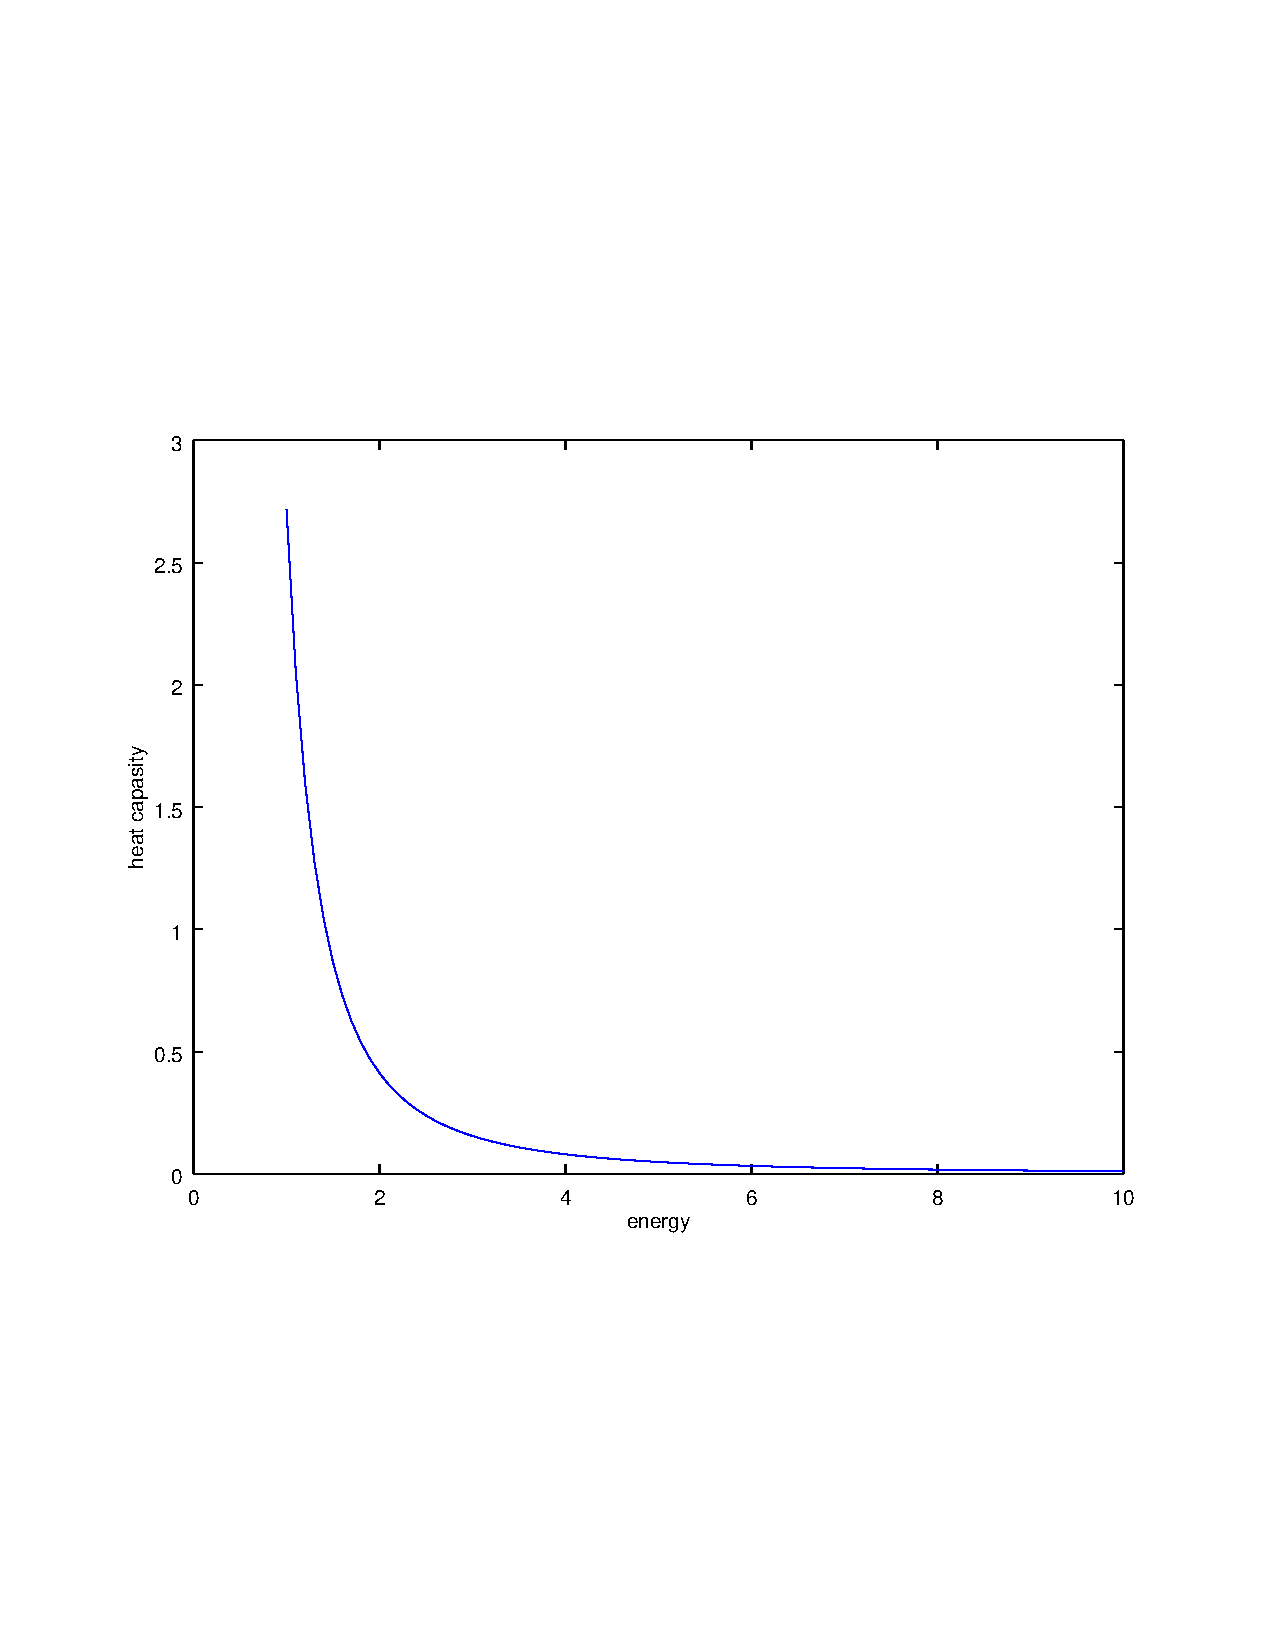
\includegraphics[scale=.6]{../octave/f1.pdf}
\end{exercise}

\begin{exercise}{3.22}
Note that $\frac{S}{k_B}\approx N\ln(N)-N_\uparrow \ln(N_\uparrow)-(N-N_\uparrow)\ln(N-N_\uparrow)$ and that $N_\uparrow=\frac{N}{2}(1-\frac{U}{N\mu B})$ and $U=-N\mu B\tanh(\frac{\mu B}{k_B T})$.  Let's plot the situation where $N=100$, in a unit system where $k_B=\mu = 1$ and leting $B=1$.\\
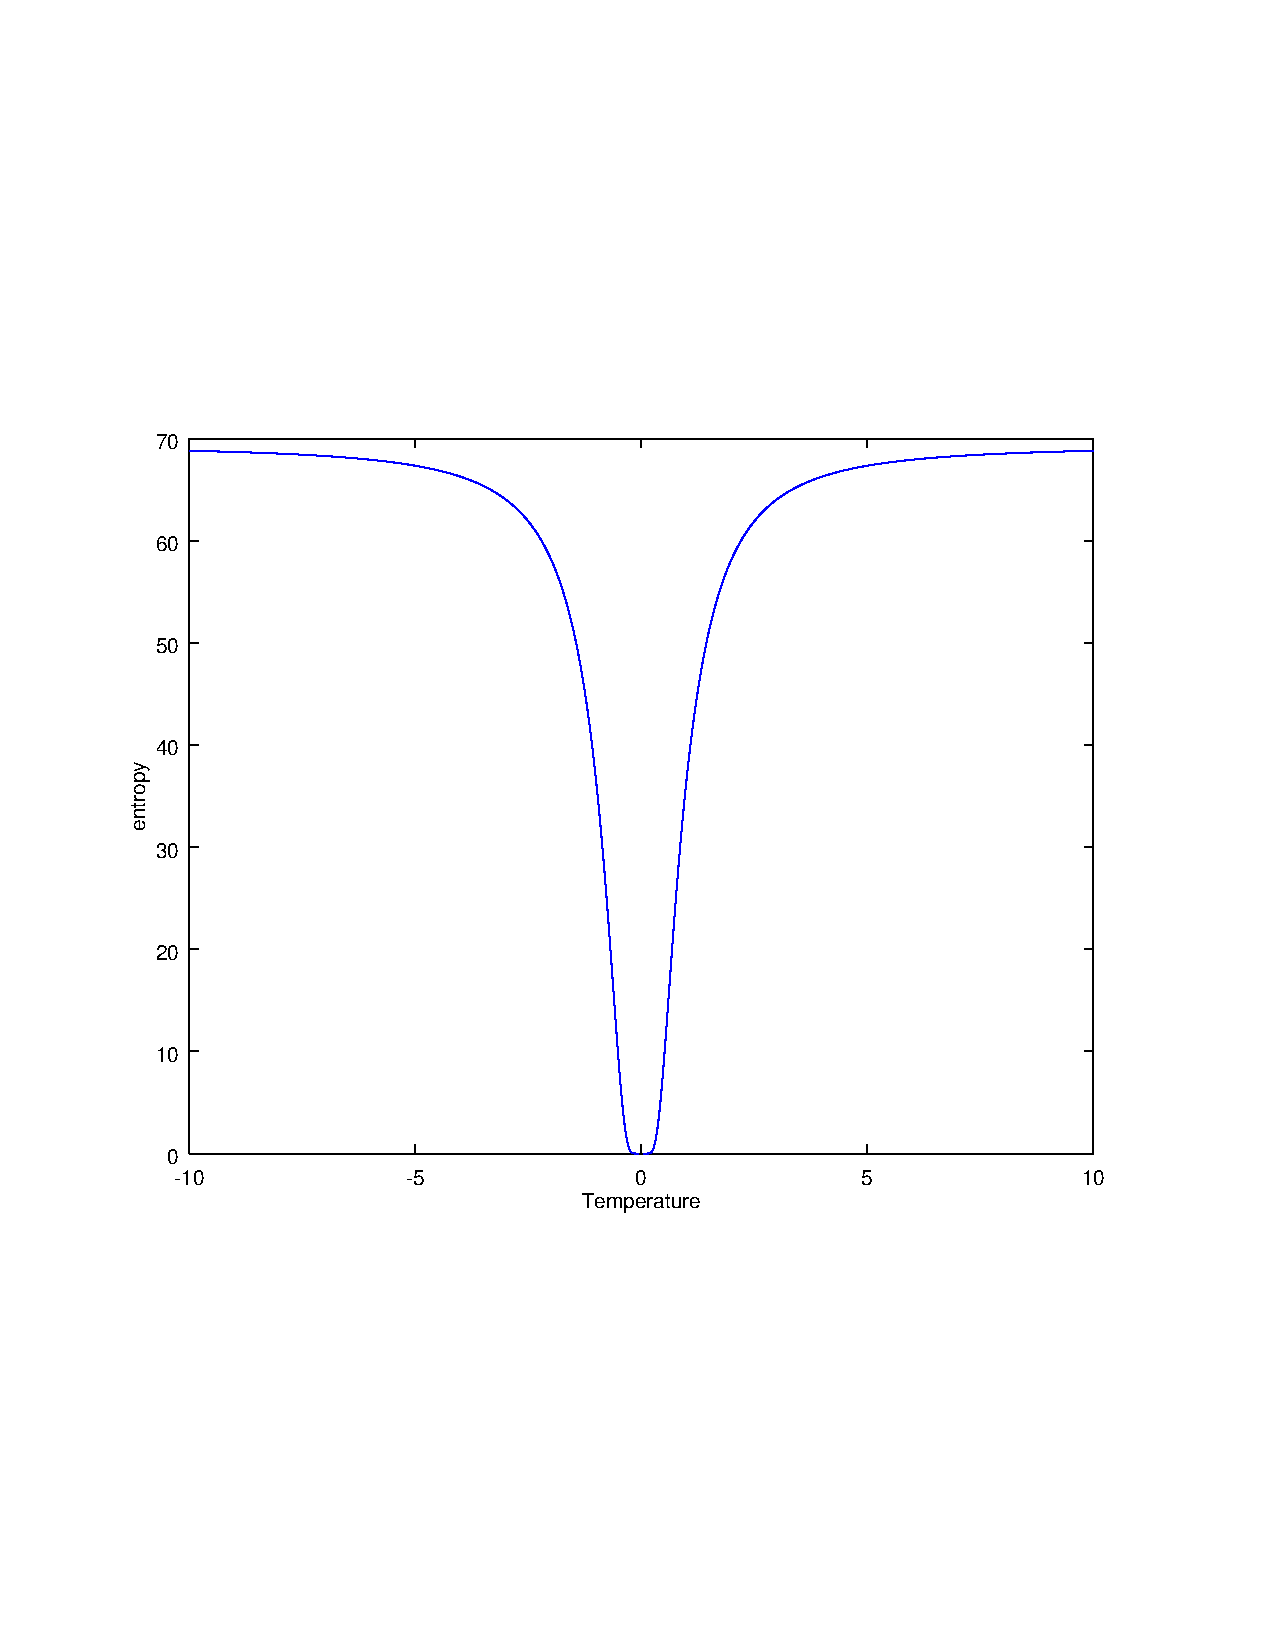
\includegraphics[scale=.6]{../octave/f2.pdf}\\
If the strength of the feald is increased the magnitude of the energy of a state will incrase and we can see by the following plot,that the magnitude of the temperature of that state will decrease.\\
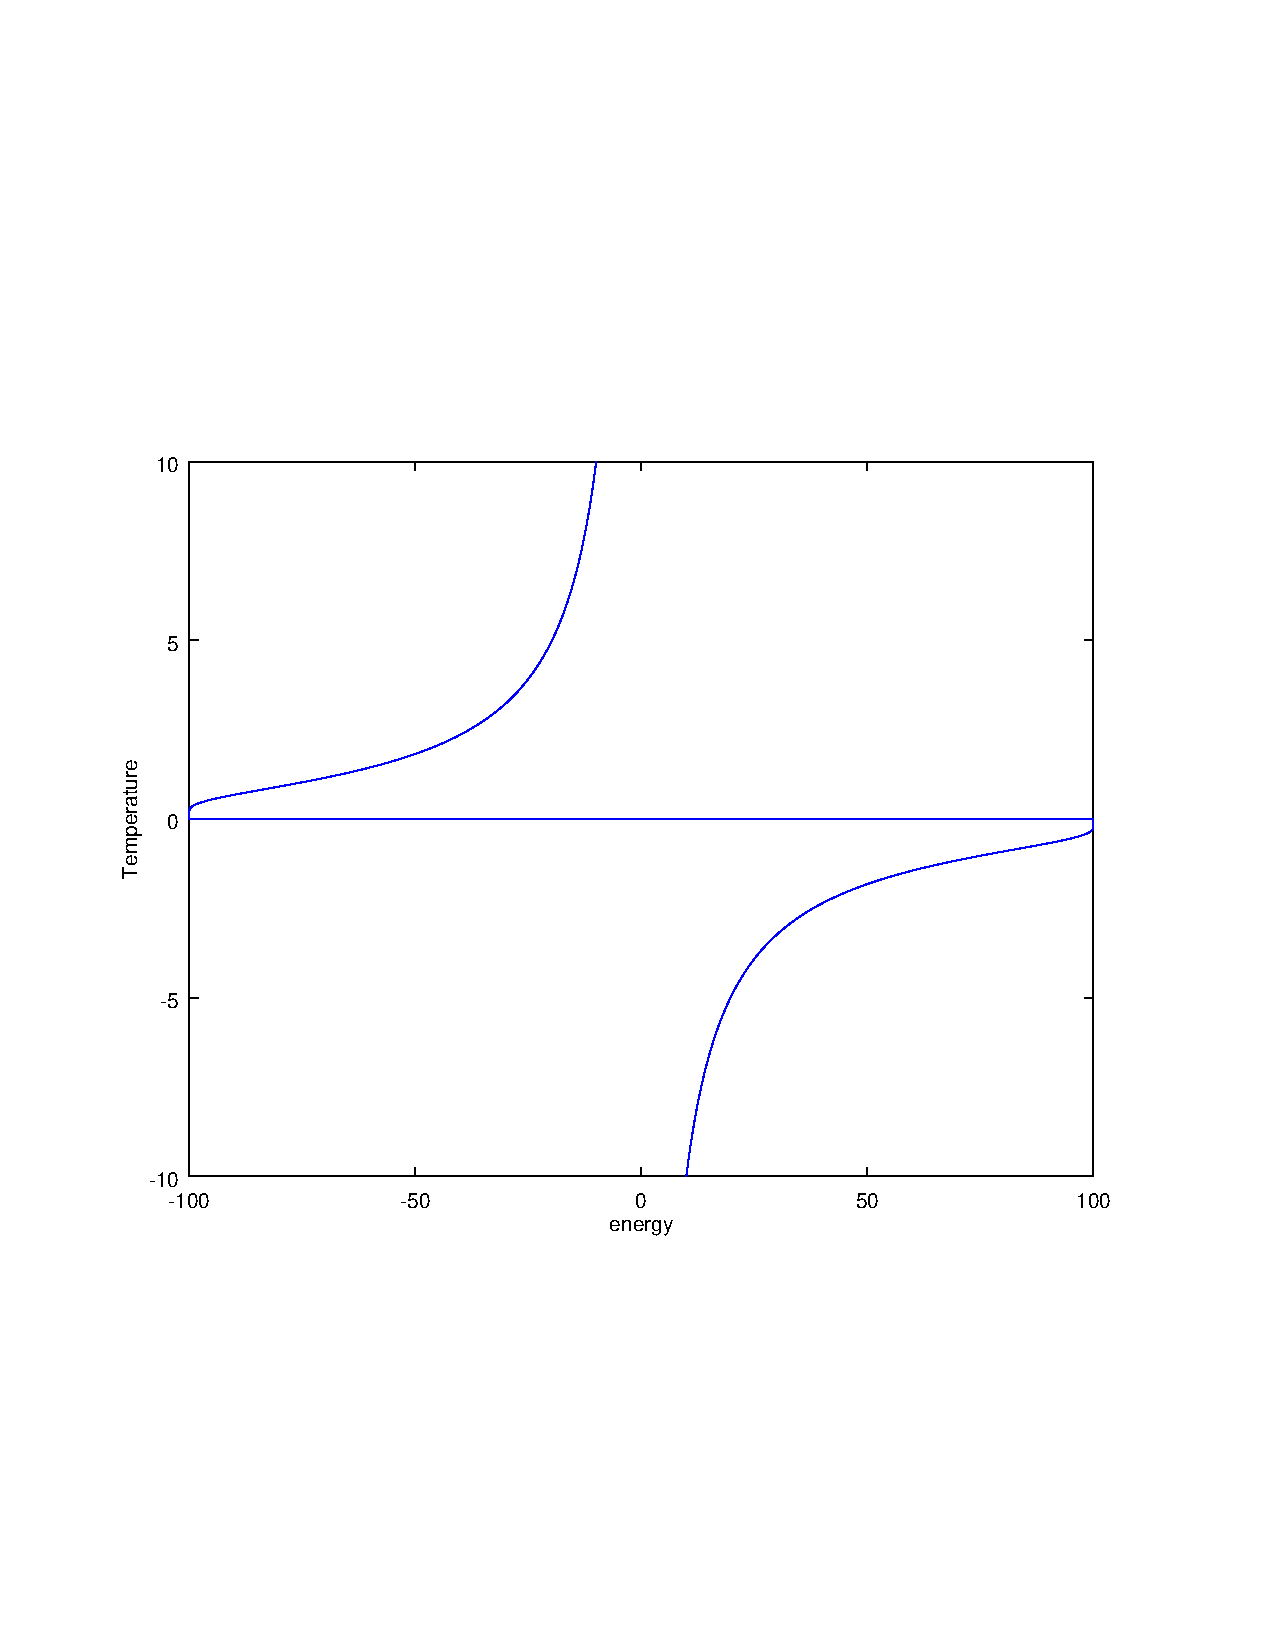
\includegraphics[scale=.3]{../octave/f3.pdf}\\
Noting that the entropy of a state is unefected by changes in the strength of the feald we see that if the temperature is increased it will simply compress the temperatur vs entropy graph along the x-axis.
\end{exercise}




\end{document}